\documentclass[tikz,border=6pt]{standalone}
\usepackage{tikz}
\usetikzlibrary{shapes,patterns}
\begin{document}
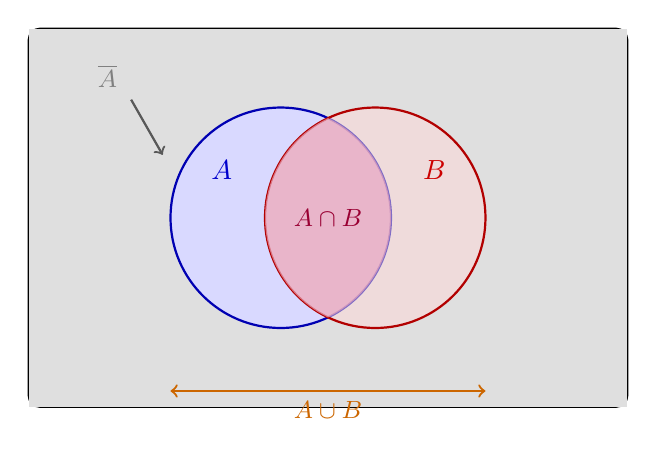
\begin{tikzpicture}[scale=1.0]
  % Sample space rectangle
  \draw[thick,rounded corners=4pt] (-3.8,-2.4) rectangle (3.8,2.4);
  \node[anchor=north east,font=\small] at (3.7,2.3) {$\Omega$};

  % Complement region shading (entire rectangle minus A)
  \begin{scope}
    \clip (-3.8,-2.4) rectangle (3.8,2.4);
    \fill[gray!25] (-3.8,-2.4) rectangle (3.8,2.4);
    \fill[white] (-0.6,0) circle (1.4);
  \end{scope}
  \node[font=\small,gray] at (-2.8,1.8) {$\overline{A}$};

  % A circle
  \draw[thick,blue!70!black,fill=blue!15] (-0.6,0) circle (1.4);
  % B circle
  \draw[thick,red!70!black,fill=red!15,fill opacity=0.5] (0.6,0) circle (1.4);

  % Intersection shading (A cap B)
  \begin{scope}
    \clip (-0.6,0) circle (1.4);
    \fill[purple!35,fill opacity=0.7] (0.6,0) circle (1.4);
  \end{scope}

  % Labels
  \node[blue!80!black,font=\bfseries] at (-1.35,0.6) {$A$};
  \node[red!80!black,font=\bfseries] at (1.35,0.6) {$B$};
  \node[purple!80!black,font=\small\bfseries] at (0,0) {$A\cap B$};

  % Union annotation (brace below circles — moved below circle bottom edges)
  \draw[<->,thick,orange!80!black] (-2.0,-2.2) -- (2.0,-2.2)
    node[midway,below,font=\small,orange!80!black] {$A\cup B$};

  % Complement label pointer
  \draw[->,gray!70!black,thick] (-2.5,1.5) -- (-2.1,0.8);
\end{tikzpicture}
\end{document}
